\chapter{Background}
\label{Chapter2}
% Main chapter title
\lhead{Chapter 2. \emph{Background}}


This chapter introduces the background and terminology necessary to understand the concepts and methods presented in this thesis. Important terms are explained in corresponding sections.

As majority of web applications' functionality is accessed through the GUI layer, it becomes customary to test important functional use-cases on the AUT through the GUI layer. Section \ref{sec:AutomatedGUITesting} gives a brief insight into automated GUI testing mechanisms.

In recent years, Selenium\footnote{\url{http://www.seleniumhq.org/}} has been a popular browser test automation tool of choice among software developers and testers. Section\ref{sec:SeleniumTesting} gives the necessary background about Selenium framework, including its implementation techniques as well as salient features.

This research leverages existing Selenium tests to capture the behavior of the AUT in terms of finite state models. For this purpose, the tool \texttt{webmate}, presented by Dallmeier et al.\cite{webmate} has been used. By leveraging existing Selenium tests, \texttt{webmate} can systematically explore the AUT to extract its behavioral usage model by implementing state-abstraction for comparing similar GUI states of the AUT. Further details about \texttt{webmate} are discussed in Section \ref{sec:WebMate}

Section \ref{sec:Statistical} presents the statistical background required to analyze the results and apply the evaluation metrics, as presented in Chapter \ref{Chapter6}.

\section{Automated GUI Testing}
\label{sec:AutomatedGUITesting}
As mentioned in Section 1, testing web applications at GUI level abstracts away finer grained internal details and helps developers to identify the undesired functionality changes in the AUT.  In comparison to traditional command-line applications or Application Programming Interfaces (APIs), automated GUI testing of modern web 2.0 applications built with multiple languages, platforms and server-side technologies poses new challenges in the areas of test-input generation, test-output verification and state space exploration.

To begin with, automatically generating and selecting inputs for a GUI is difficult since depending upon the type of the application, different applications might require specific combinations of inputs and values. 
Current practices for automated test input generation include techniques such as symbolic execution\cite{Ganovetal}, using random input generation\cite{godefroid2005dart} or search based techniques\cite{gross2012search}. However, automated input generation is not trivial for a web applications, since the GUI test automation tool needs to be aware of the context of the AUT. Although test inputs can be generated using functional specifications, concrete specifications along with different input combinations may not be available in practice and desired functional coverage of the AUT is not achieved. Thus in many cases, input generation is often left to the test developer to explore the desired states of the AUT hidden behind input forms and elements.

In addition, even in cases when a testing tool can generate different input combinations automatically, it still needs to verify the correct behavior of the AUT. This is usually done by applying appropriate test assertions and oracles on the test outputs\cite{Baresi:Oracles}. Mechanisms such as using Capture/replay tools\cite{joshi2006capture} require the tester to first manually capture the behavior of the AUT by performing different GUI-level events, recording them and storing the expected output as a part of the test-case. In the replay phase, recorded tests are replayed on the AUT and the output is checked against the captured textit{expected output} to assert the application behavior. Such approach requires manual effort to record each test and is not suitable for regression testing as every time the AUT changes, there is a need to re-record the tests in order to generate new expected outputs. 

Moreover, as the size of the AUT increases, the number of possible actions on the GUI increases exponentially. This is especially an issue in case of regression testing since as possible number of paths and sequences increases, covering the entire possible number of state space and executions becomes infeasible.

On the other hand, as opposed to the automated crawlers, humans possess the domain knowledge of the AUT required to generate valid test inputs and apply precise oracles on the test outputs, many developers often choose to identify the core functionality of the AUT and automate their regression tests using frameworks such as Selenium, as detailed in Section 2.2.

\section{Test automation using Selenium}
\label{sec:SeleniumTesting}
\subsection{Architecture}
\label{ssec:webdriverArchitecture}
Selenium is a browser automation framework designed to automate the system testing of web applications. While the Selenium project offers a different set of tools depending upon the type of application, the  \texttt{webdriver}\footnote{\url{http://www.seleniumhq.org/projects/webdriver/}} project is of particular the interest for laying the foundation of this thesis. The \texttt{webdriver} project provides an API to test dynamic web 2.0 applications. 

The \texttt{webdriver} API supports various modern programming languages such as Java, Python, C\#, Ruby, PHP etc. by providing language level bindings along with a set of browser specific drivers. Figure \ref{fig:webdriverArchitecture} gives an overview of the architecture of Selenium \texttt{webdriver}.

The API \textit{drives} (controls) the browser in a manner that it emulates all possible end users interactions with the browser, such as clicks, form-inputs, drag-drops, file uploads etc. Selenium \texttt{webdriver} tests can thus explore the possible set of functionalities of the AUT. As an example, Snippet \ref{code1} illustrates a \texttt{webdriver} test case (Java) to test the \textit{login} functionality of AUT as depicted in Figure \ref{fig:a}.
\begin{center}
\begin{scriptsize}
\centering
\lstset{
  basicstyle=\ttfamily,
  columns=fullflexible,
  keepspaces=true,
%   frame=none,
}
% \verb|basicstyle=\ttfamily, columns=fullflexible, keepspaces=true|
  
\begin{lstlisting}[caption=Login test,label=code1]
public void loginTest(){
driver.get("http://www.application-under-test.com");
driver.findElement(By.id("uname")).sendKeys("user");
driver.findElement(By.id("pwd")).sendKeys("passwd");
driver.findElement(By.linkText("Login")).click();
}
\end{lstlisting}
\end{scriptsize} 
\end{center}
 
\begin{figure}[h!]
\makeatletter 
% \renewcommand{\thefigure}{\@arabic\c@figure}
\makeatother
    \centering
  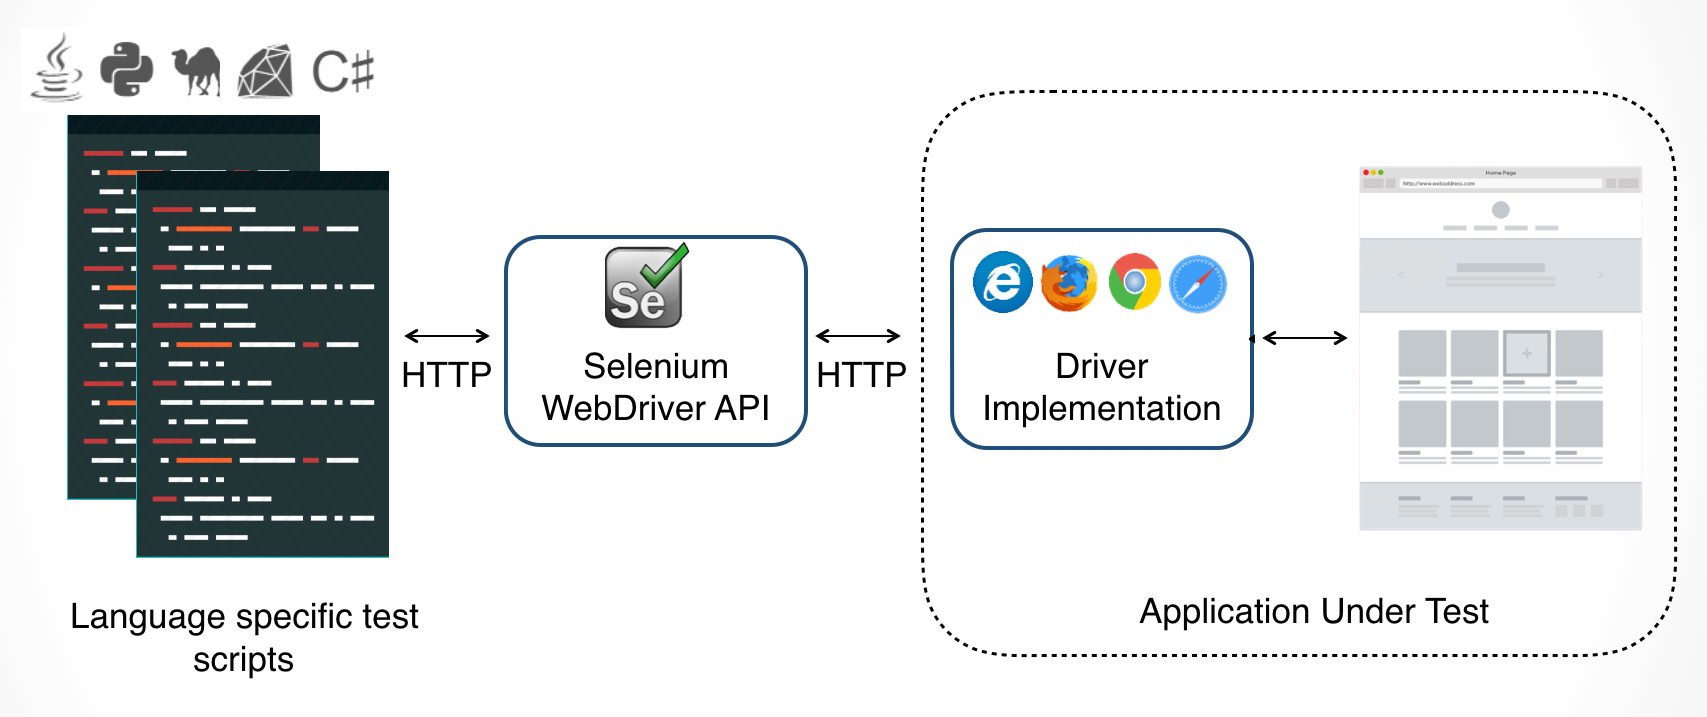
\includegraphics[width=5.5in,height=2.2in]{./Figures/webdriver_Archi}
  \caption{Selenium \texttt{webdriver} architecture}
  \label{fig:webdriverArchitecture} 
\end{figure}

The \texttt{webdriver} API communicates with the browser specific driver using a common wire protocol. The protocol transfers the test-commands written in language specific bindings to the browser specific driver in the form of UTF-8\footnote{\url{https://tools.ietf.org/html/rfc3629}} encoded JSON\footnote{\url{http://www.json.org/}} data. The API uses HTTP\footnote{\url{https://www.w3.org/Protocols/}} as a transport mechanism to transfer these commands to the driver and to return the response from the driver to the language specific code. 
\noindent 
Following example illustrates the communication between the language specific test-commands (Java in this case) and the \texttt{RemoteWebDriver} through \texttt{webdriver} API :
\begin{enumerate}
\item The client (test-script) requests the URL of the AUT.\\
\begin{small}
\texttt{driver.get("http://www.application-under-test.com");}
\end{small}
\item This command is translated as a JSON object to be transferred using the wire protocol as following:\\
\begin{small}
\texttt{\{"url": "http://www.application-under-test.com"\}}
\end{small}
\item The JSON object is then sent over HTTP (using POST\footnote{\url{http://tools.ietf.org/html/rfc7231\#section-4.3.3}} request in this case). To identify and associate each request/response session uniquely to the session-specific commands, \texttt{webdriver} uses a unique handle in terms of the \textit{SessionId}\footnote{\url{https://w3c.github.io/webdriver/webdriver-spec.html\#sessions}}\\
\begin{small}
\texttt{Method : POST, Path: session/{session-id}/url}\\
\end{small}
The resultant URL is :\\
\begin{small}
\texttt{http://localhost:7055/hub/session/{session-id}/url}
\end{small}
\end{enumerate}

Each browser specific driver implementation such as the \texttt{Firefox Driver}\footnote{\url{https://code.google.com/p/selenium/wiki/FirefoxDriver}} or the \texttt{RemoteWebDriver}\footnote{\url{https://code.google.com/p/selenium/wiki/RemoteWebDriver}} has its own mechanism for carrying out the above-mentioned communication. 

The \texttt{RemoteWebDriver} implementation provides the capability to run the Selenium tests against a remote machine. In essence, \texttt{RemoteWebDriver} is comprised of a client-server architecture, where client is the language specific test-case and and server is a simple Java servlet. The \texttt{RemoteWebDriver} servlet acts as a multiplexer, by connecting the client to the specific browser(s) and system configurations requested by the client. The browser and other configurations are provided in terms of capabilities, via command-line or directly from the language specific code.

\subsection{Locating UI Elements}
\label{ssec:locatingUIElements}
In order to locate GUI elements such as input forms, buttons, checkboxes etc. in the DOM (Document Object Model), \texttt{webdriver} specifies \textit{``Find Element''} and \textit{``Find Elements''} methods for locating a single element and a list of elements, respectively. Within the scope of these methods it is also possible to traverse the DOM tree to locate the \textit{Child Elements} i.e. children nodes of a parent element in the tree. Each language specific binding has its own command to invoke these methods by providing the UI-element locator object, such as\begin{small} HTML\end{small} \texttt{id}, the \texttt{css selector} or \texttt{xpath} expressions.

\begin{verbatim}
\#Classification : STRUCTURAL VS NON-STRUCTURAL
\#ADVANTAGE/PROPERTIES IN SHORT
\#IMPLEMENTATION EXAMPLE,
\end{verbatim}

The most commonly  used\footnote{\url{http://www.seleniumhq.org/docs/03_webdriver.jsp\#locating-ui-elements-webelements}} UI locators and their implementation in Java is listed as following:
\begin{itemize}
% ### ID
\item 
By \texttt{id}:
Locates the UI Element using \texttt{id} attribute of \begin{footnotesize} HTML\end{footnotesize} element.
\newline
\begin{footnotesize}
\framecolorbox[\linewidth][l]{gray}{white}{\texttt{<input id="login" type="button"/>}}
\texttt{WebElement loginButton = driver.findElement(By.id("login"));
}
\end{footnotesize}
% Locating UI Elements using unique HTML \texttt{id} attributes is the most preferred and reliable method\footnote{\url{http://www.seleniumhq.org/docs/03_webdriver.jsp\#by-id}}.  
% #NAME
\item 
By \texttt{name}:
Locates the UI Element using \texttt{name} attribute of \begin{footnotesize} HTML\end{footnotesize} element.
\newline
\begin{footnotesize}
\framecolorbox[\linewidth][l]{gray}{white}{\texttt{<input type="button" name="login"/>
}}
\texttt{WebElement loginButton = driver.findElement(By.name("login"));
}
\end{footnotesize}
% #Class name
\item 
By \texttt{class name}:
Locates the UI Element using the value of \begin{footnotesize} HTML\end{footnotesize} \texttt{class} attribute.
\newline
\begin{footnotesize}
\framecolorbox[\linewidth][l]{gray}{white}{\texttt{<input type="button" class="login"/>
}}
\texttt{WebElement loginButton = driver.findElement(By.className("login"));
}
\end{footnotesize}

% #tag name
\item 
By \texttt{tag name}:
Locates the UI Element using the \begin{footnotesize} HTML\end{footnotesize} \texttt{tag} attribute.
\newline
\begin{footnotesize}
\framecolorbox[\linewidth][l]{gray}{white}{\texttt{<button name="login"</button>
}}
\texttt{WebElement loginButton = driver.findElement(By.tagName("button"));
}
\end{footnotesize}

% #link text
\item 
By \texttt{link text}:
Locates the UI Element using the visible text of the hyperlink.
\newline
\begin{footnotesize}
\framecolorbox[\linewidth][l]{gray}{white}{\texttt{<a href="\#">Login</a>}}
\texttt{WebElement loginButton = driver.findElement(By.linkText("Login"));
}
\end{footnotesize}

% # partial link text
\item 
By \texttt{partial link text}:
Locates the UI Element by partial matching of visible text of the hyperlink.
\newline
\begin{footnotesize}
\framecolorbox[\linewidth][l]{gray}{white}{\texttt{<a href="\#">Login Here</a>}}
\texttt{WebElement loginButton = driver.findElement(By.partialLinkText("Login"));
}
\end{footnotesize}
% # CSS
\item 
By \texttt{css selector}:
Locates the UI Element using the \texttt{css selector} representing the \begin{footnotesize} HTML\end{footnotesize} \texttt{tags, name, class and id} attributes through various combinations.\texttt{css selectors} also allow locating parent and children nodes of a DOM tree. 
\newline
\begin{footnotesize}
\framecolorbox[\linewidth][l]{gray}{white}{\texttt{<input id="login"/>
}}
\texttt{WebElement loginButton = driver.findElement(By.cssSelector("input\#login"));
}
\end{footnotesize}
% # xpath
\item 
By \texttt{xpath}:
Locates the UI Element using the \texttt{xpath} expressions as it supports navigating XML as well as xHTML element tree.Similar to \texttt{css selectors}, the \texttt{xpath} expressions also allow locating parent and children nodes of a DOM tree. 
\newline
\begin{footnotesize}
\framecolorbox[\linewidth][l]{gray}{white}{\texttt{<input id="login"/>
}}
\texttt{WebElement loginButton = driver.findElement(By.xpath("//input[@id="login"]"));
}
\end{footnotesize}
\end{itemize}
Depending upon the GUI structure of AUT and the applicability of UI element locators, different location strategies can be used in combination. The Influence of these UI locator strategies on the robustness of Selenium tests is discussed in Chapter \ref{Chapter4}.
% (https://w3c.github.io/webdriver/webdriver-spec.html#sessions)

\section{WebMate}
\label{sec:WebMate}
As mentioned in Chapter \ref{Chapter1}, \texttt{webmate}\cite{webmate} is a system-level automated testing and analysis framework. Primarily developed as a cross-browser compatibility testing tool,\texttt{webmate} supports different browsers and platforms. It can leverage existing Selenium tests in order to remote control the browser to interact with the dynamic web 2.0 applications involving JavaScript and Ajax elements. 

By leveraging the Selenium tests, \texttt{webmate} explores the AUT and extracts a behavioral usage-model. The usage-model is essentially a finite state automaton which captures the exploration graph of the different actions performed by the Selenium test on the AUT. 

Figure \ref{fig:webmateArchitecture} gives an example of \texttt{webmate} leveraging the \texttt{loginTest} (Snippet \ref{code1}) to generate the usage-model. For security reasons, Selenium tests are integrated with \texttt{webmate} inside a virtual machine. The virtual machine hosts a Selenium hub\footnote{\url{http://www.seleniumhq.org/docs/07_selenium_grid.jsp}} infrastructure, along with a set of browsers. Existing Selenium tests can be executed with \texttt{webmate} by using the \texttt{RemoteWebDriver} capabilities, such as by specifying browser name, security credentials for \texttt{webmate} etc. \texttt{webmate} generates the usage-model without affecting the underlying Selenium tests.

The states of the usage-model correspond to different states of the GUI and the transitions correspond to different interactions with the AUT such as clicks, form-inputs etc. For each state of the usage-model, \texttt{webmate} is able to record its visual (GUI) state, in the form of a screen-shot of the AUT. \texttt{webmate} makes it possible to recognize functional differences (e.g. missing button) by assessing the usage models to compare GUI state and trace level differences. Due to these features of \texttt{webmate}, it is used as a tool of choice in this thesis for establishing the ground truth for the robustness analysis, as detailed in Chapter \ref{Chapter6}

\begin{figure}
\makeatletter 
% \renewcommand{\thefigure}{\@arabic\c@figure}
\makeatother
    \centering
  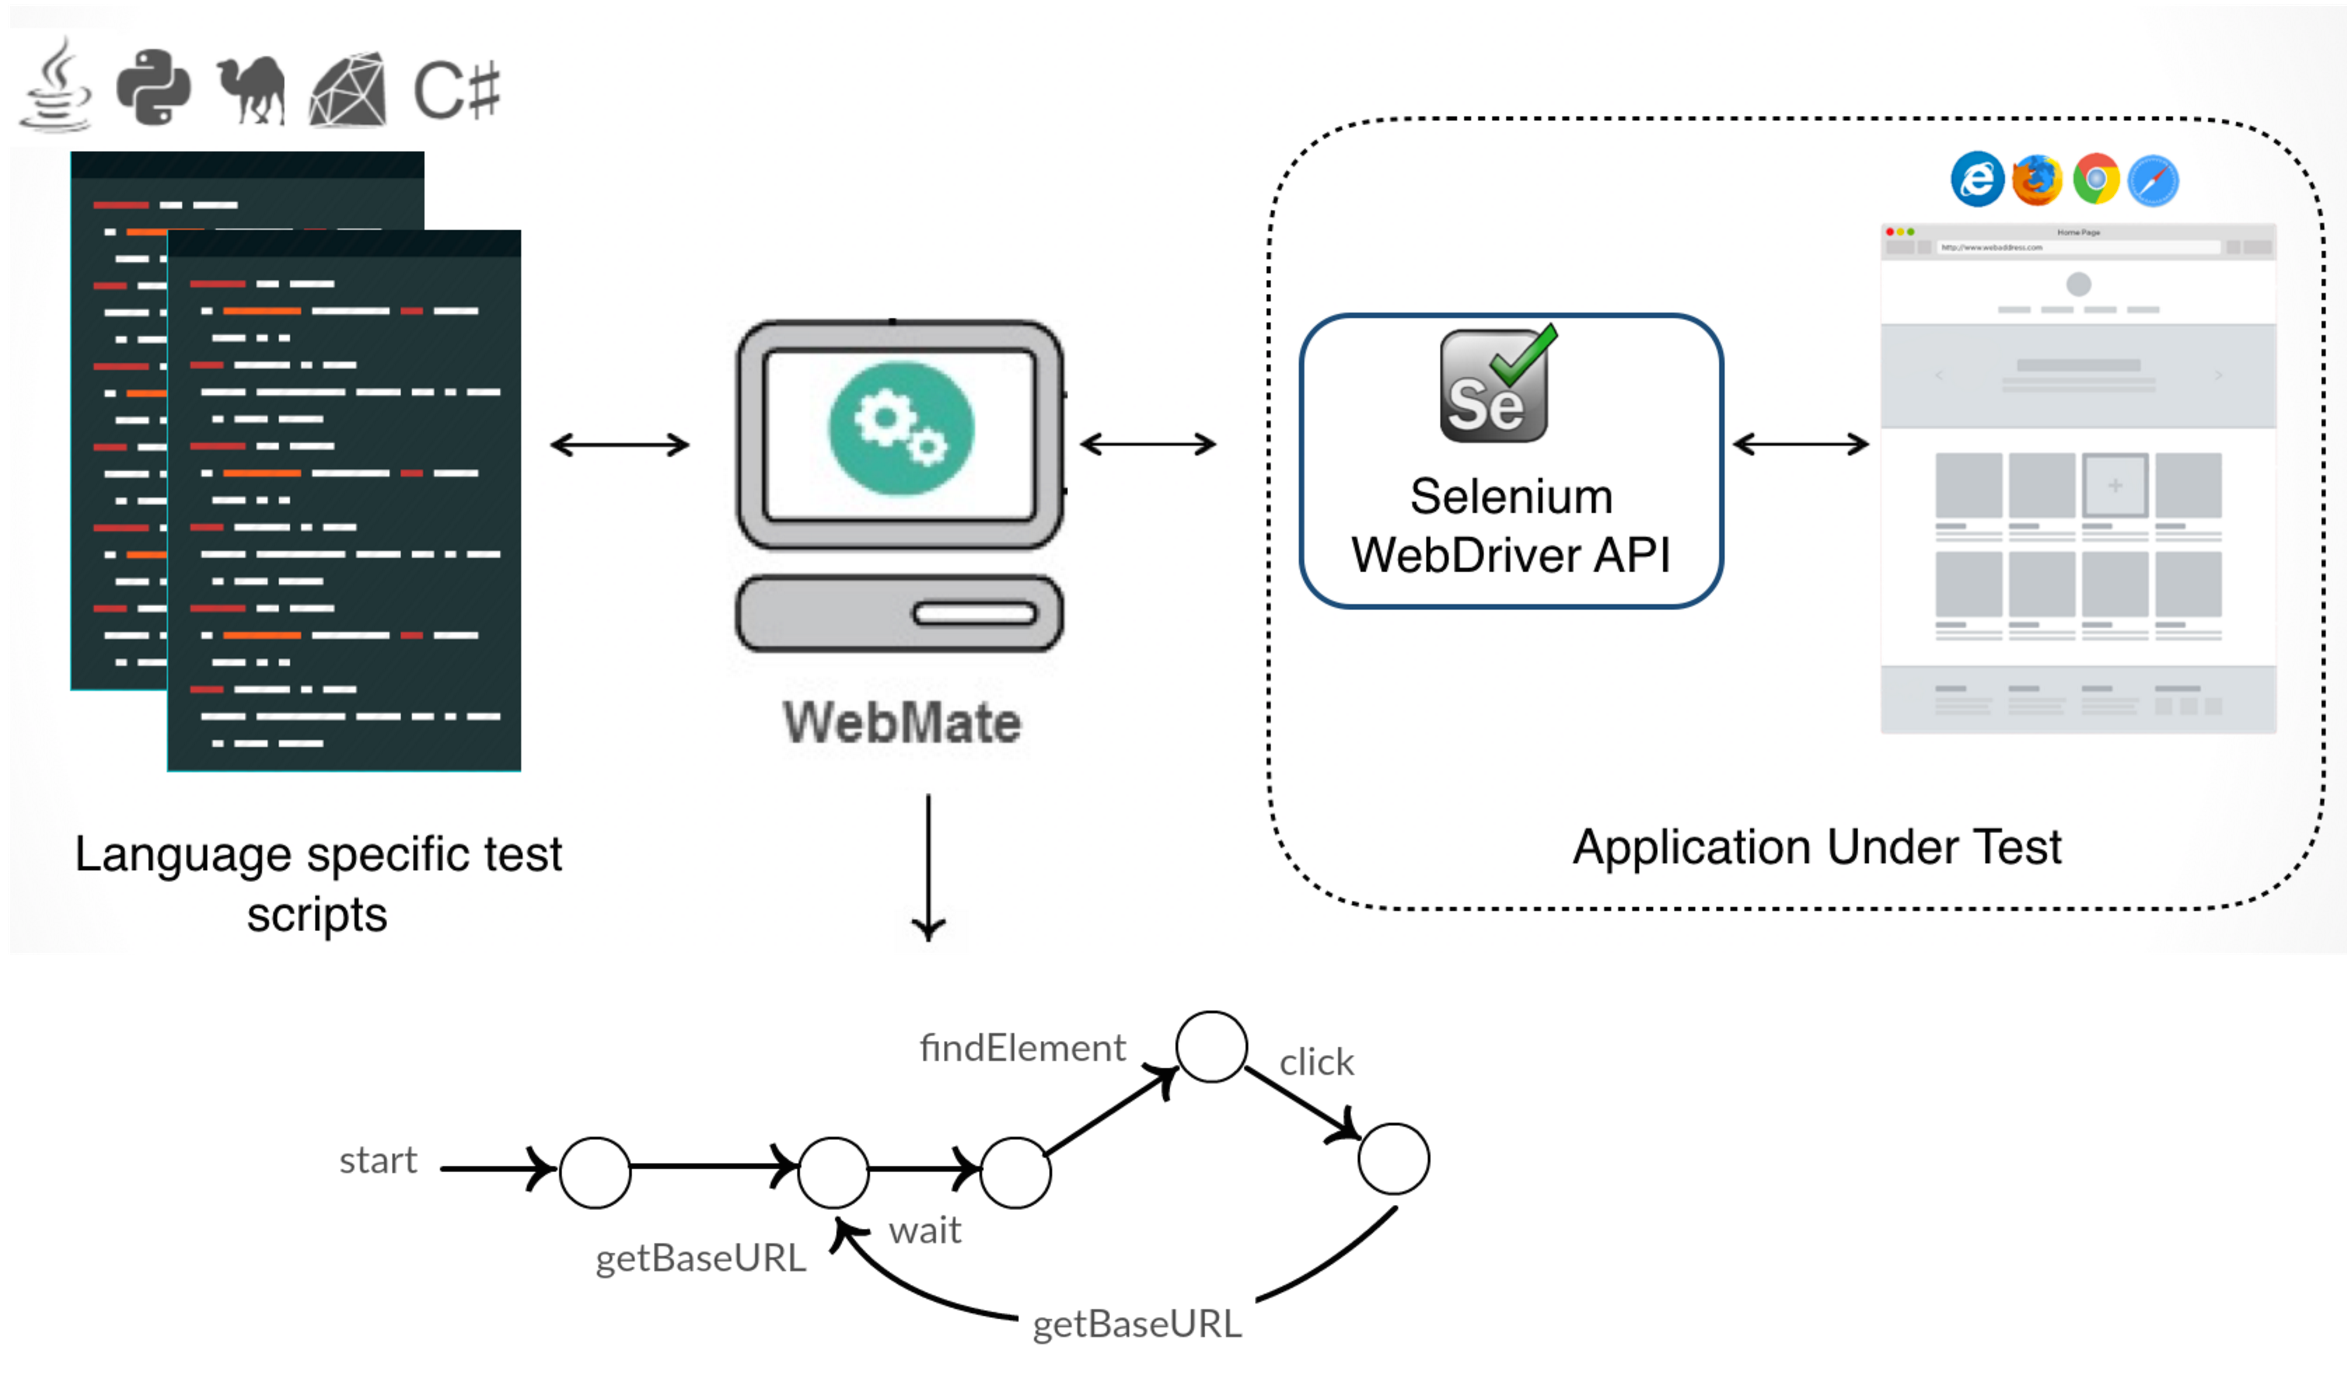
\includegraphics[width=5.5in,height=3in]{./Figures/webmate-state-graph}
  \caption{Webmate architecture}
  \label{fig:webmateArchitecture} 
\end{figure}

\section{Automated Parallel Deployment}
\label{sec:autoDeployment}
To test and evaluate different versions of AUT, it is necessary to make these versions accessible for the Selenium testing setup. It is possible to install and deploy these versions locally since most of the open-source application vendors make older versions of their applications available for public usage. This is either done by releasing packaged binaries ready to deploy, such as \texttt{war} files for Java applications or by checking out the code from version control repositories such as git, subversion, mercurial etc.

In order to expedite this process, we aim to deploy multiple versions of the AUT in parallel, on a remote server such as a Linux based virtual machine. Figure \ref{fig:deployment} depicts the overview of remote automatic deployment process; three versions of the AUT are running simultaneously against their individual database instances.
\section{Statistical Background}
\label{sec:Statistical}